\chapter{Architecture Overview} \label{chap:Architecture}
In this chapter, I discuss the overall architecture, underpinning the trail running website created. In section \ref{graphQlSection} I describe the use of GraphQl as the technology behind the server side API and why I decided to use this over the more widely used REST architectural style.

To provide this website to the user, we follow the popular client server architecture \cite{wiki:ClientServerModel}. The Map Interface described in \ref{mappingPlatform} is provided to the client using Angular, a fronted framework explained in section \ref{frontendFramework}. The server is provided using the new GraphQl API described in \autoref{graphQlSection}.



\section{Overview}
The client of the web application (including the trail interface described in chapter \ref{chap:TrailInterface}) are created with Angular. The client sends to and retrieves data from a GraphQl Server. The GraphQl Server is connected to a MySQl database. Prisma provides a GraphQl \acrfull{dal} to simplify access to the data stored in the database. This overall structure can be seen in \autoref{fig:graphArchitecture}.

\begin{figure}[ht]
    \centering
    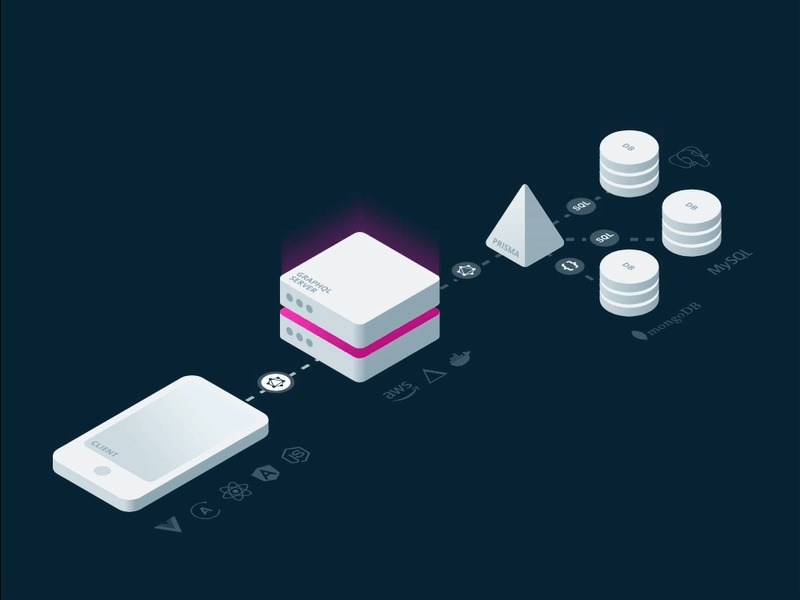
\includegraphics[width=\textwidth]{graphql-architecture.jpg}
    \caption{Overall Architecture of the web application}
    \label{fig:graphArchitecture}
\end{figure}

Our server responds with data written in \acrfull{json} format.

\section{Authentication and Authorisation}
Authentication, Authorisation  are a crucial part of Identification any web application s to ensure the users can only interact data intended for them. Moreover, it is needed to allow users to be able to login to the system. The system provides authentication and authorisation with the power of \acrfull{jwt}.

\acrshort{jwt} is a compact open standard (RFC 7519), that allows the secure transmission of tokens between two parties in  \acrshort{json} format \cite{jones2015json}. The information shared between the two parties is digitally signed, and hence can trusted between be verified and trusted by the parties \cite{auth02019json}. This gives us a lightweight way of providing authentication and authorisation between the client on our user and the server.

Each user has a unique email they add when they sign-up as defined in our schema seen in appendix \autoref{app:graphqlSchema}. When a user, attempts to log in with their email (which is unique to each user) we find the user in the database and their user ID. Once the Id is found we digitally sign the user ID using the standard \acrfull{hs256} and a secret. As the system is the only one that knows the secret, this ensures integrity. This token is then sent the the client and the client can store this token locally.

Whenever the client needs to authorise themselves, the client sends the request information (such as a query) and the token as part of the Authorisation header. The server reads the token from the header and can use that to verify client, granting them authorisation when needed.

\section{Necessary \acrshort{crud} operations}
\acrfull{crud} are the four basic operations that most web applications need to provide \cite{codeacademy2019crud}. They are self explanatory verbs that provide the essential operations user's need to be able to interact with web applications.

\subsection{Uploading a Trail}
When a user creates a trail using the map interface described in \autoref{chap:TrailInterface}, it is persisted to the server to be stored in the database. The information needed to be stored for trails are the name of the trail (for identification and searching), points and the lines that are used to create the trail (including the elevation and distance information). We store the points and lines to be used to redraw the trail on the map interface when presenting it to the user. A user can have multiple created trails

\subsection{Exploring Trails}
Exploring trails is how users can find new trails. The main way users can explore trails is via the Recommender system discussed in \autoref{chap:Recommender}. The system also provides other methods to allow users to find trails.

\subsubsection{Sorted Ranked List of Trails}
On the main explore page, there are tabs displaying trails in sorted ranked list. Although in \autoref{subsec:WhyRecSystems}, we discuss the importance of using Recommender systems to suggest trails, the Recommender system is slightly ineffective with new users who are yet to run a trail. Hence we provided other methods of ranking trails to the user.

\begin{itemize}
    \item \textbf{Popular trails:} Trails sorted in descending order of the number of users who run the trail (i.e. trails with the most runs are ranked at the top). 
    \item \textbf{Top rated trails:} Trails sorted in descending order of the average rating from users who run the trail.
    \item \textbf{Recently added trails:} Trails sorted in descending order of the date they where created.
\end{itemize}

\subsubsection{Real time Search}
Users should also be able to search for specific trails and users. The system offers the capability of real time searches of trails and users. To do this, they server will need to be queried as the user types in the search string, creating a performance bottleneck. Angular comes built in with a technology called RxJs that allows us to alleviate this bottleneck.

RxJs is a Javascript library from ReactiveX built on the Reactive programming paradigm \cite{wan2000functional}. It's an API for asynchronous programming with observable streams \cite{reactivex2018main}. It allows us to treat our user input as data streams, that we can subscribe to and manipulate before sending the request to the server. ReactiveX provides us with operators to help improve the efficiency of our real time search.

\begin{figure}[htb!]
    \centering
    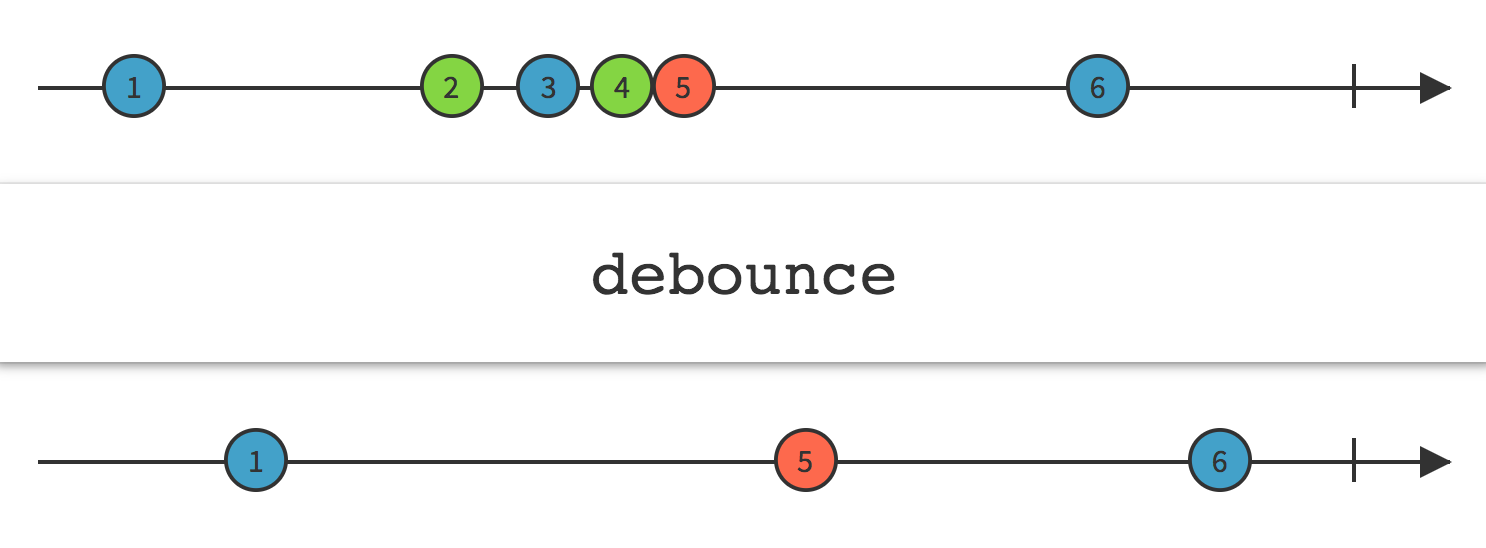
\includegraphics[width=\textwidth]{debounce-time.png}
    \caption{Debounce Time Operator}
    \label{fig:debounceTime}
\end{figure}

\begin{figure}[htb!]
    \centering
    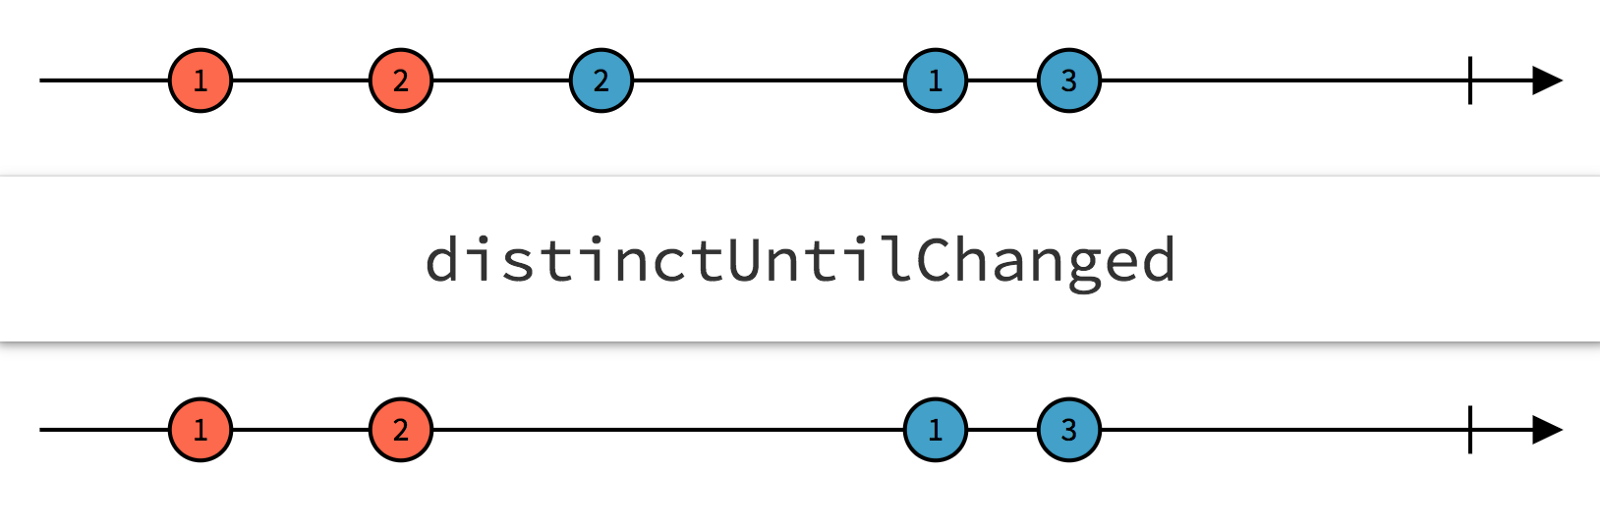
\includegraphics[width=\textwidth]{distinctUntilChanged.png}
    \caption{Distinct until changed}
    \label{fig:distinctUntilChanged}
\end{figure}


\subsection{Feed page}

\subsection{Prisma Layer}
Prisma\footnote{\url{https://www.prisma.io/}} is a data access layer that replaces traditional ORM's\footnote{Object Relational Mappings}. It sits in front of databases and provides methods that allow the server to access the database. The main feature that it provides is the Prisma Client, which is an auto-generated type-safe database client that creates the data access layer.

\section{Frontend Framework} \label{frontendFramework}
There are 2 main way's to build modern web applications. It can be done using native web stack of HTML, CSS and Javascript or (and more popularly), built using modern web application frameworks. Although there are many proponents to building with the native web stack, modern applications, such as this one, are more complex in nature and hence, require tools make it easier to build complex solutions. They also have big communities and strong documentation that make debugging easier \cite{medium:WhyModernJSFrameworkExist}.

There are a large variety Frontend Frameworks out there. I considered the most popular ones which where
\begin{itemize}
    \item Angular \footnote{\url{https://angular.io/}}
    \item React \footnote{\url{https://reactjs.org/}}
    \item Vue.js \footnote{\url{https://vuejs.org/}}
\end{itemize}

The framework I decided on was Angular. This was because it has excellent and well-detailed documentation, it came out of the bag with all most of the tools I needed to get started with (I didn't need alot of external libraries at the start), and it used Typescript over Javascript.

Typescript \footnote{\url{https://www.typescriptlang.org/}} is a super set \footnote{it is built on top of Javascript} of Javascript, created by Microsoft that provides optional but strict type checking, making developing large scale applications easier \cite{bierman2014understanding}. It also allows me to combine Javascripts functional programming paradigm \cite{hughes1989functional}, with an Object oriented programming paradigm.

\subsection{State Management With Redux}
One of the main problems that comes with building web applications is managing state in the frontend. On the editor page, where user's create and trails, It is important to manage the state of the application to allow users to undo and redo any changes they make when creating or editing Trails.

It is possible to create your own system to manage state in angular using systems such as Angular's Dependency Injection \cite{wiki:DependencyInjection}, however this does not suffice to handle applications with alot of interaction. It also doesn't provide standard support for recording user interactions and a means of replaying those steps when needed.

Redux is javascript library created by Facebook use for managing state in user interfaces \cite{wiki:Redux}. NgRx \cite{cheng2018state} is a framework built on the fundamentals of Redux\footnote{The Flux Architecture}, to enable us to maintain state in our Application. It is provides a functional way of building Reactive Applications.

NgRx comes with dev tools as shown in figure \ref{fig:reduxDevTools}. It allows us to track the state of our application as it evolves from initial login, to router navigations and trail changes. This record can then be used to rewind through previous actions, allowing us to provide undo and redo functionalities to the user.
\begin{figure}[ht]
    \centering
    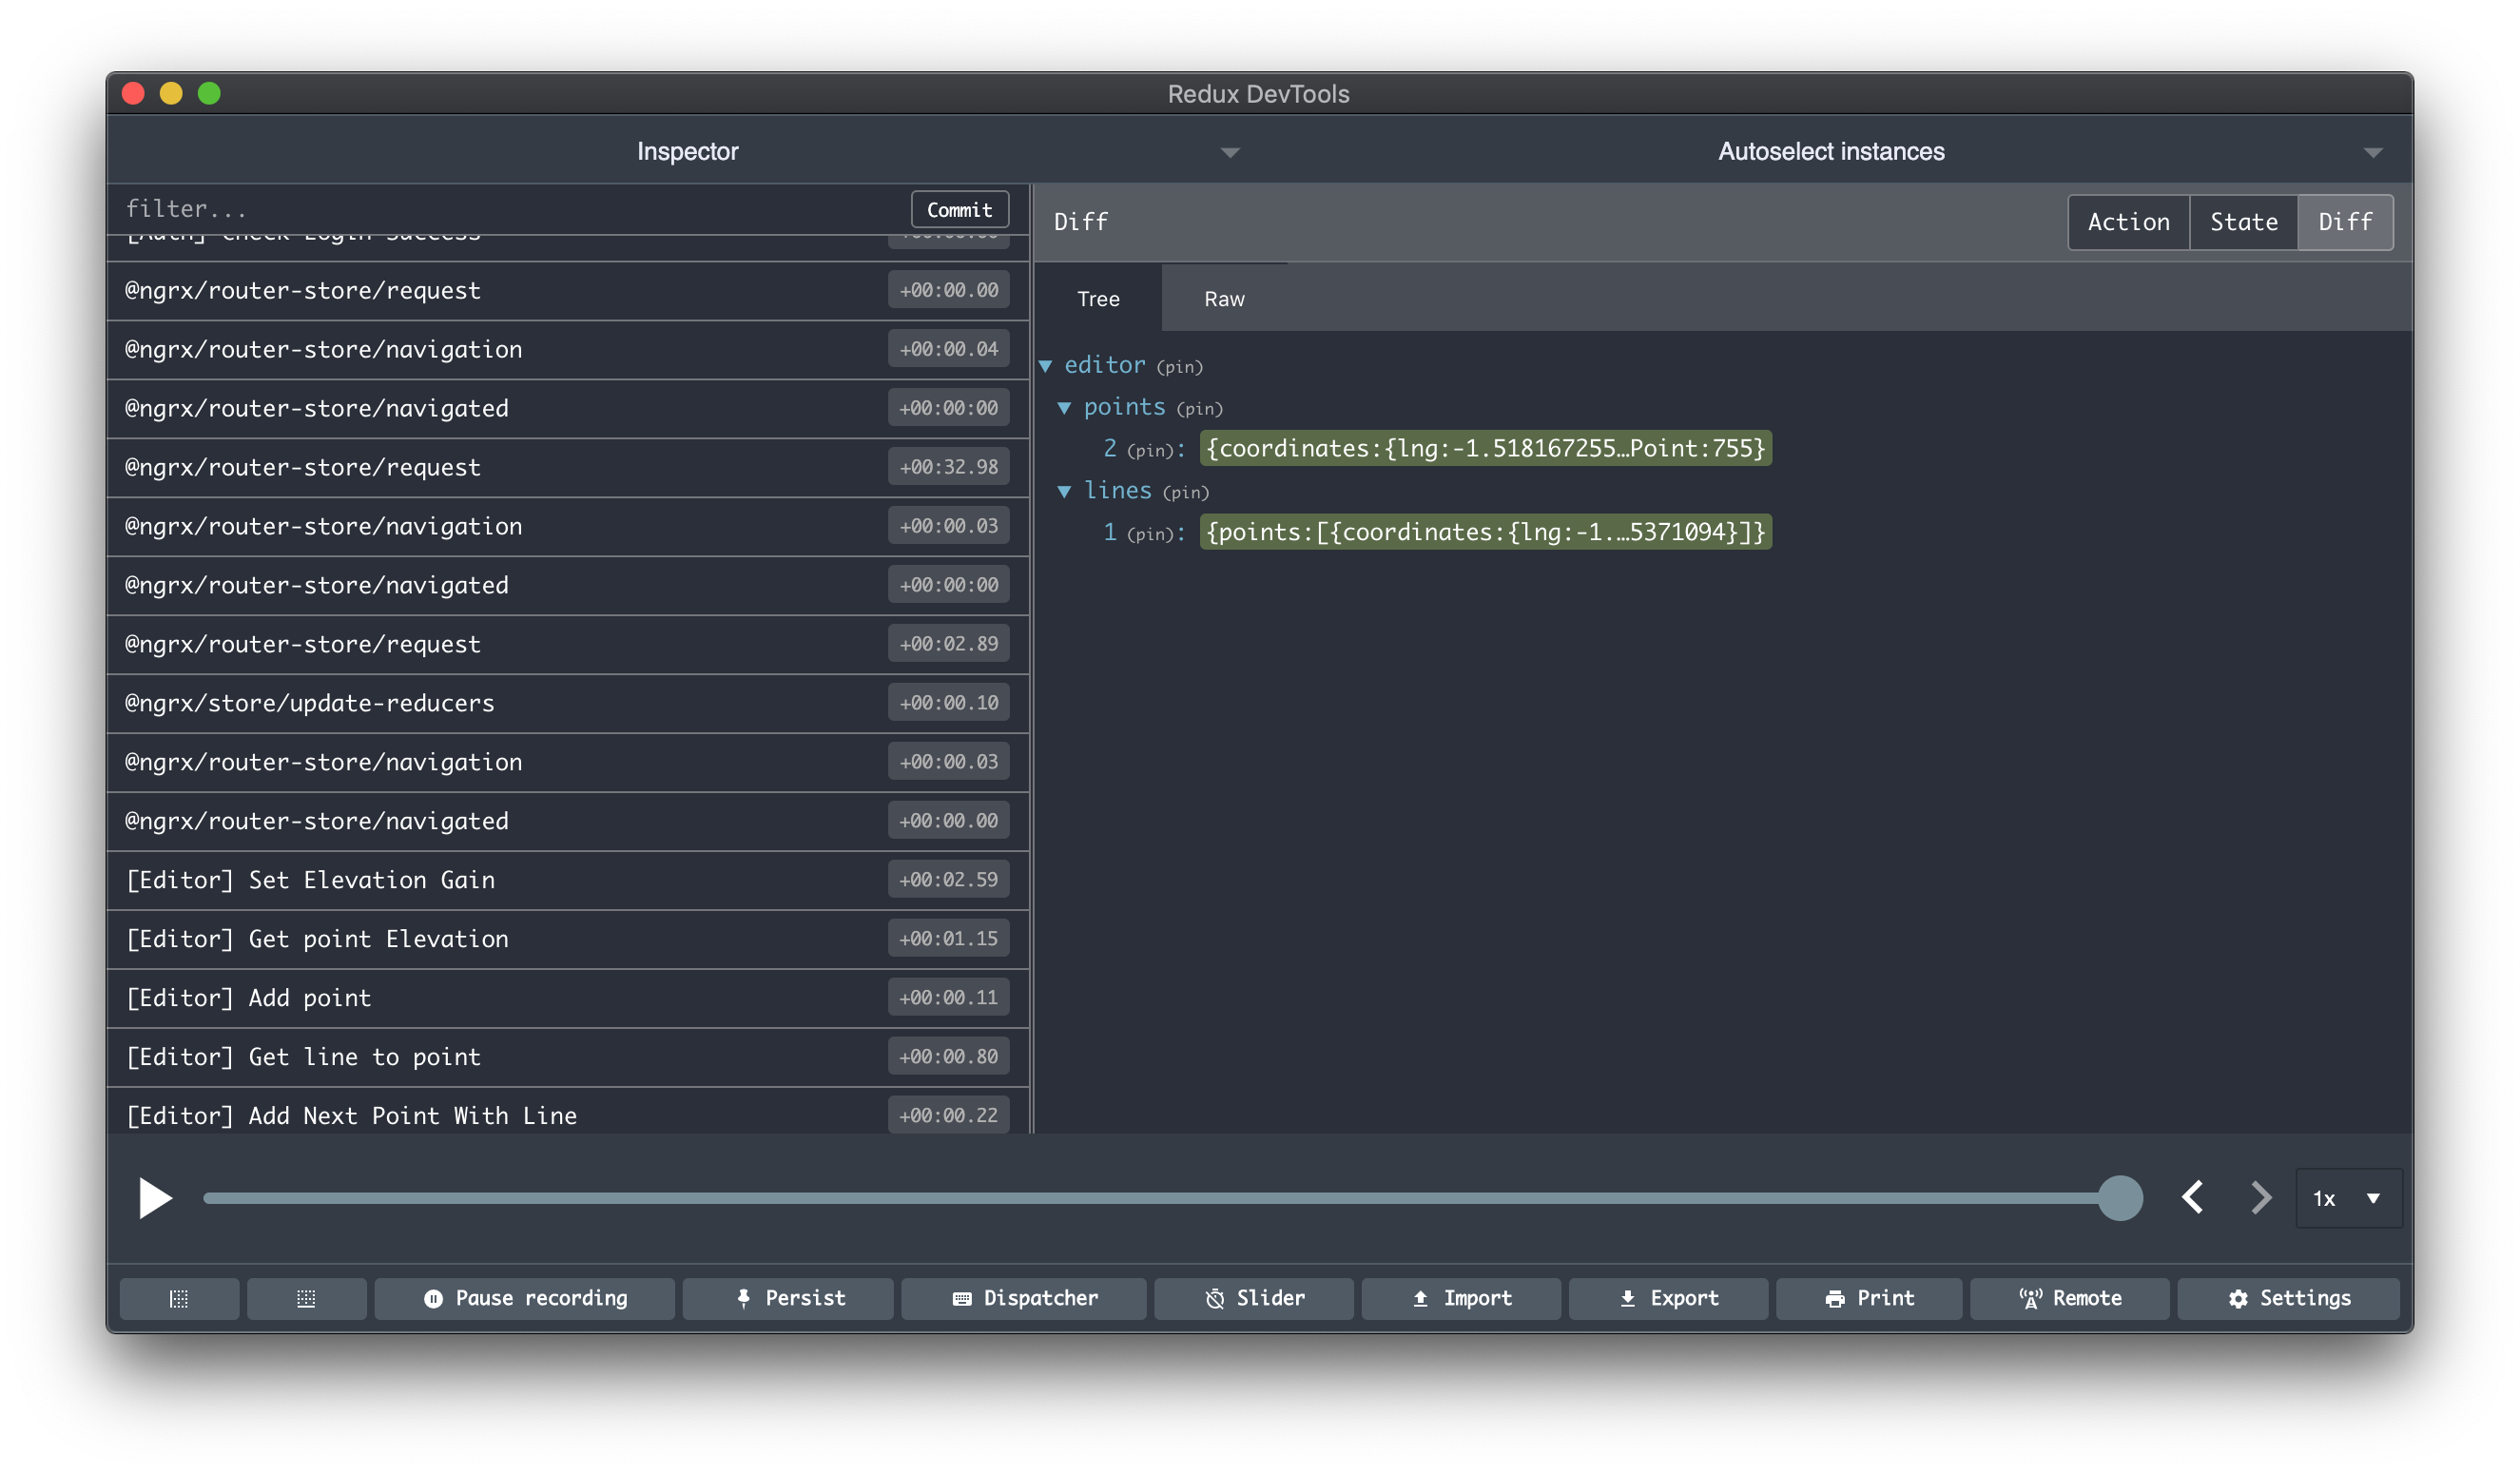
\includegraphics[width=\textwidth]{redux-dev-tools.png}
    \caption{Redux Dev Tools}
    \label{fig:reduxDevTools}
\end{figure}

\subsection{Realtime Search with RxJs}
Real time searching is an important feature that allows users to find results to queries as they type such a query. To do this, we need to query the database (or cache) on every keystroke. However this is a massive performance bottleneck on both the server as it is will be queried too often and the client as it would have to render the results of the that's been returned on each key stroke.

We can use Reactive programming and the power of ReactiveX\footnote{http://reactivex.io/} to help mitigate these problems. ReactiveX is an API for asynchronous programming with Obsever Patterns. What it does is it allow's us to listen to input from user in the form of data streams. We can then apply various functions to the query as we get it before we send the query off to the server. 

What I do is to call the function \textit{debounceTime}, which waits a given amount of time after a user types in the query before emitting the data. Every time the user starts retyping during this time, the stream is paused again until the queries the user stops typing. That way we can still simulate real time results.

Another function we use is \textit{distinctUntilChanged}, which prevents the stream from emitting any values until the value being emitted is different from the previous value. This has to be done after \textit{debounceTime}.

\section{Facilitating Competition}
To promote competition, users can upload runs for a route. When users upload a run, they also have to upload a time on. On the trail description page, these runs are displayed and sorted in time order to form a leaderboard as shown in image \ref{fig:leaderboard8}

\begin{figure}[ht]
    \centering
    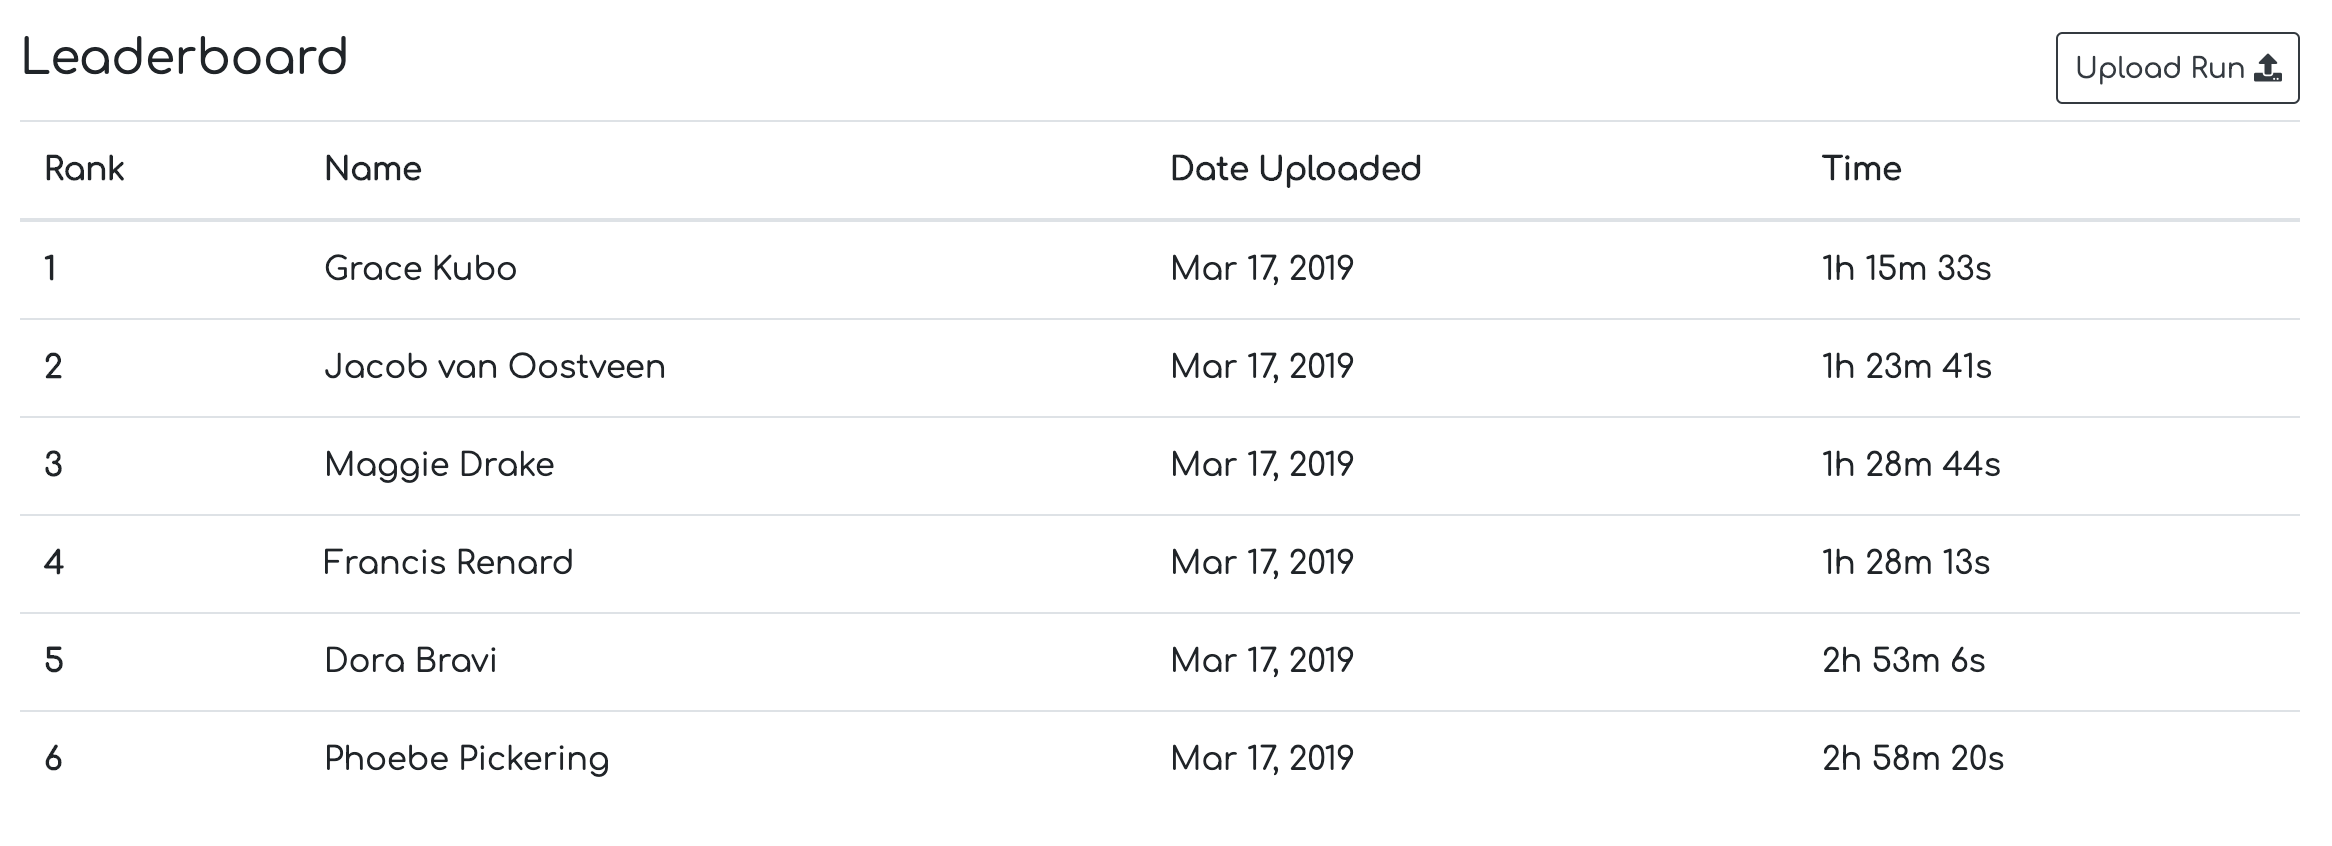
\includegraphics[width=\textwidth]{leaderboard.png}
    \caption{Leaderboard System}
    \label{fig:leaderboard8}
\end{figure}